\documentclass[10pt,a4paper, margin=1in]{article}
\usepackage{fullpage}
\usepackage{amsfonts, amsmath, pifont}
\usepackage{amsthm}
\usepackage{graphicx}
\usepackage{float}

\usepackage{tkz-euclide}
\usepackage{tikz}
\usepackage{pgfplots}
\usepackage{pdfpages}

\pgfplotsset{compat=1.13}

\usepackage{geometry}
 \geometry{
 a4paper,
 total={210mm,297mm},
 left=10mm,
 right=10mm,
 top=10mm,
 bottom=10mm,
 }
 % Write both of your names here. Fill exxxxxxx with your ceng mail address.
 \author{
  Adıgüzel, Gürhan İlhan\\
  \texttt{e2448025@ceng.metu.edu.tr}
  \and
  İçen, Anıl\\
  \texttt{e2448488@ceng.metu.edu.tr}
}

\title{CENG 384 - Signals and Systems for Computer Engineers \\
Spring 2023 \\
Homework 1}

\begin{filecontents}{q3.dat}
  n  xn
 -8  0
 -7  3
 -6  0  
 -5  0
 -4 -4
 -3  0
 -2  2
 -1 -1
  0  0
  1  -1
  2  0
  3  0
  4  3
  5  0
\end{filecontents}

\begin{filecontents}{q5.dat}
  t  xn
  1  1
  3  -3
  4  1
\end{filecontents}

\begin{document}
\maketitle

\noindent\rule{19cm}{1.2pt}

\begin{enumerate}

\item %write the solution of q1
    \begin{enumerate}
    \vspace{25}
    \item %write the solution of q1a
        \\ Given  $z = x + yj$ and  $2z + 5 = j - \bar{z}$, finding $\bar{z}$ which is conjugate of z :
        \\  Applying the $z$ and $\bar{z}$ to the given equation:
        \\ $2(x+ yj)+5 = j – (x–yj) $
        \\ $(2x+5) + 2yj = -x + (y+1)j$   
        \\ $ 2x+5  = -x$
        \\ $y+1 = 2y$
        \\ So $ x = -5/3$ and $y = 1$
        \\ Putting the values $x$ and $y$ in the $z$
        \\  $z= -5/3 + j$
        \\\\$|z| = \sqrt{1 + 25/9} = \sqrt{34/9}$ 
        \\\\$|z|^2  = 34/9 $
        \\ \begin{tikzpicture}
            \begin{scope}[thick,font=\scriptsize]
            \draw [->] (-3,0) -- (3,0) node [above left]  {$\Re\{z\}$};
            \draw [->] (0,-3) -- (0,3) node [below right] {$\Im\{z\}$};
            \iffalse% Single
            % If you only want a single label per axis side:
            \draw (1,-3pt) -- (1,3pt)   node [above] {$1$};
            \draw (-1,-3pt) -- (-1,3pt) node [above] {$-1$};
            \draw (-3pt,1) -- (3pt,1)   node [right] {$i$};
            \draw (-3pt,-1) -- (3pt,-1) node [right] {$-i$};
            \else% Multiple
            % If you want labels at every unit step:
            \foreach \n in {-2,...,-1,1,2}{%
                \draw (\n,-3pt) -- (\n,3pt)   node [above] {$\n$};
                \draw (-3pt,\n) -- (3pt,\n)   node [right] {$\n i$};
            }
            \fi
            \end{scope}
            \draw [red, line width=0.8] (0, 0) -- (-5/3, 1) node [left, red] {$z = -5/3 + j$};
        \end{tikzpicture}
    \vspace{25}
    \item %write the solution of q1b
        \\ Given $z = re^{j\theta}$ :  
        \\$z^{5} = r^{5}e^{j5\theta} = 32j$
        \\ This equation give us $r=2$
        \\ Remembering the equation $(e^{j\theta} = cos(\theta) + jsin(\theta))$ : 
        \\$(e^{j5\theta} = j =  cos(\pi/2) + jsin(\pi/2))$
        \\ Therefore : 
        \\ $5\theta = \pi/2$
        \\ $\theta = \pi/10$
        \\ z in polar form:
        \\\\ $z = 2(cos(\frac{\pi}{10}) + jsin(\frac{\pi}{10}))$
        \\\\ $z = 2e^{(j{\frac{\pi}{10}} + \frac{\pi}{5}k)}$ where $k = 1,2,3...$
    \newpage
    \item %write the solution of q1c
        \\ Multiplying both numerator and denominator of given $z$ with $(1+j)$:
        \\\\ $z = \frac{j-\sqrt{3}}{-2} = \frac{\sqrt{3}-j}{2}$
        \\\\ Finding the magnitude r and angle $\theta$ of $z$:
        \\\\ $r = \sqrt{(\frac{\sqrt{3}}{2})^{2} + (\frac{-1}{2})^{2}} $
        \\\\ $r = 1$
        \\ $\theta = tan^{-1}(\frac{-1}{\sqrt{3}})$
        \\ $\theta = \frac{-\pi}{6}$
        \\
    \item %write the solution of q1d
        \\ $ j = e^{j\frac{\pi}{2}}$
        \\ $ z = e^{j\frac{\pi}{2}} * e^{-j\frac{\pi}{2}} $
        \\ $ z = e^{j\frac{\pi}{2}} * e^{-j\frac{\pi}{2}} = 1 $
        \\ $ z = 1 + 0j$ 
        \\
    \end{enumerate}
    
\item %write the solution of q2  
    Below is the signal for $y(t) = x(\frac{1}{2}t + 1)$
        \begin{figure}[H]
            \centering
                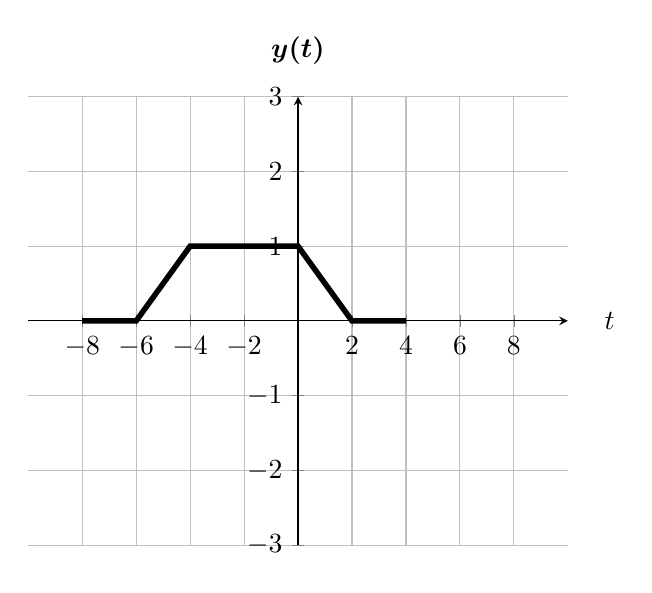
\begin{tikzpicture}[scale=1.0]
                    \begin{axis}[
                      axis lines=middle,
                      xlabel={$t$},
                      ylabel={$\boldsymbol{y(t)}$},
                      xtick={-8, -6, -4, -2, ..., 8},
                      ytick={-3, -2, -1, ..., 3},
                      ymin=-3, ymax=3,
                      xmin=-10, xmax=10,
                      every axis x label/.style={at={(ticklabel* cs:1.05)}, anchor=west,},
                      every axis y label/.style={at={(ticklabel* cs:1.05)}, anchor=south,},
                      grid]
                    \path[draw,line width=2pt] (-8,0) -- (-6,0) -- (-4,1) -- (0,1) -- (2,0) -- (4,0);
                   \end{axis}
                \end{tikzpicture}
                \caption{$t$ vs. $y(t)$.}
                \label{fig:q2}
        \end{figure}

\item %write the solution of q3
    \begin{enumerate}
    \item %write the solution of q3a
        Below is the signal for $x[-n] + x[2n - 1]$
        \begin{figure}[H]
            \centering
            \begin{tikzpicture}[scale=1.0] 
              \begin{axis}[
                  axis lines=middle,
                  xlabel={$n$},
                  ylabel={$\boldsymbol{x[-n]+x[2n-1]}$},
                  xtick={ -9, -8, ..., 6},
                  ytick={-4, -3, -2, -1, ..., 4},
                  ymin=-4, ymax=4,
                  xmin=-9, xmax=6,
                  every axis x label/.style={at={(ticklabel* cs:1.05)}, anchor=west,},
                  every axis y label/.style={at={(ticklabel* cs:1.05)}, anchor=south,},
                  grid,
                ]
                \addplot [ycomb, black, thick, mark=*] table [x={n}, y={xn}] {q3.dat};
              \end{axis}
            \end{tikzpicture}
            \caption{$n$ vs. $x[-n]+x[2n-1]$.}
            \label{fig:q3}
        \end{figure}

    \item %write the solution of q3b
        \\ $x[-n] + x[2n-1]$ in terms of the unit impulse function is as follows:   
        \\ $3\delta(n+7)-4\delta(n+4)+2\delta(n+2)-\delta(n+1)-\delta(n-1)+3\delta(n-4)$
    \end{enumerate}
    
\newpage
\item %write the solution of q4
    \begin{enumerate}   
    \item %write the solution of q4a
        \\$x(t) = 5sin(3t - \frac{\pi}{4})$ 
        \\This is a continuous signal, fundamental period can be found as:
        \begin{align*}
        \\T&=\frac{2\pi}{\omega} 
        \\T&=\frac{2\pi}{3}  
        \end{align*}
        \\$\frac{2\pi}{3}$ is the fundamental period of $x(t)$.
        \\
    \item %write the solution of q4b
        \\$x[n] = cos[\frac{13\pi}{10}n] + sin[\frac{7\pi}{10}n ]$ 
        \\ A discrete signal is periodic only if $\omega_0 = 2\pi$ $m/N$ for some integers $N>0$ and $m$.
        \\Fundamental period for $cos[\frac{13\pi}{10}n]$ (Since this is a discrete signal we need an integer $m$ to make $N$ integer):
        \begin{align*}
            \\N_1&=\frac{2\pi}{\Omega}m 
            \\N_1&=\frac{2\pi}{\frac{13\pi}{10}}m 
            \\N_1&=\frac{20}{13}m \ \ \ \ \ \ m = 13 
            \\N_1&=20
        \end{align*}
        \\Fundamental period for $sin[\frac{7\pi}{10}n]$ (Since this is a discrete signal we need an integer $m$ to make $N$ integer):
        \begin{align*}
            \\N_2&=\frac{2\pi}{\Omega}m 
            \\N_2&=\frac{2\pi}{\frac{7\pi}{10}}m 
            \\N_2&=\frac{20}{7}m \ \ \ \ \ \ m = 7 
            \\N_2&=20
        \end{align*}
        \\To be able to find fundamental period for $x[n]$ we need to find $lcm(N_1,N_2)$:
        \begin{align*}
            \\N &= lcm(N_1,N_2) 
            \\N &= lcm(20,20) 
            \\N&=20
        \end{align*}
        \\20 is the fundamental period of $x[n]$.
        \\
    \item %write the solution of q4c 
        \\$x[n] = \frac{1}{2}cos[7n-5]$ 
        \\This is also a discrete signal fundamental period can be found as:
        \begin{align*}
            \\N&=\frac{2\pi}{\Omega}m 
            \\N&=\frac{2\pi}{7}m
        \end{align*}
        \\There does not exist any integer $m$ which can make $N=\frac{2\pi}{7}m$ integer, so we can exactly say $x[n]$ is an aperiodic signal. 
        \\
    \end{enumerate}

\newpage
\item %write the solution of q5
    \begin{enumerate}
    \item %write the solution of q5a
        \\ Unit step function of $x(t)$ is:
        \\ $x(t) = u(t-1) - 3u(t-3) + u(t-4)$
        \\
    \item %write the solution of q5b
        \\We know that $\delta$(t) = $\frac{du(t)}{dt}$
        \\Therefore, we can find $\frac{dx(t)}{dt}$ from the unit step function found above. 
        \\\\$\dfrac{dx(t)}{dt} = \dfrac{d(u(t-1) - 3u(t-3) + u(t-4))}{dt}$
        \\\\$= \dfrac{du(t-1)}{dt} - 3\dfrac{du(t-3)}{dt} + \dfrac{du(t-4)}{dt}$
        \\\\$= \delta(t-1) - 3\delta(t-3) + \delta(t-4) $

    \begin{figure}[H]
            \centering
            \begin{tikzpicture}[scale=1.0] 
              \begin{axis}
                [
                  axis lines=middle,
                  xlabel={$t$},
                  ylabel={$\frac{dx(t)}{dt}$},
                  xtick={ -1, 0, ..., 6},
                  ytick={-4, -3, -2, -1, ..., 3},
                  ymin=-4, ymax=3,
                  xmin=-1, xmax=6,
                  every axis x label/.style={at={(ticklabel* cs:1.05)}, anchor=west,},
                  every axis y label/.style={at={(ticklabel* cs:1.05)}, anchor=south,},
                  grid,
                ]
                \addplot [ycomb, black, thick, mark=*] table [x={t}, y={xn}] {q5.dat};
              \end{axis}
            \end{tikzpicture}
            \caption{$\frac{dx(t)}{dt}$.}
            \label{fig:q5}
        \end{figure}
    \end{enumerate}    
    
\vspace{50}    
\item %write the solution of q6
    \begin{enumerate}
    \item %write the solution of q6a
        \\$y(t) = tx(2t+3): $
        \\
        \begin{enumerate}
            \item
            \\$Memory: $
            System does not need memory since it does not need to use neither past inputs. So this system is memoryless.
            \\
            \item
            \\$Stability: $
            The system is not stable since when we change $x(t)$ with a constant, we can see output is not constant.
            \\
            \item
            \\\\$Causality: $
            The system does not depend on only past and present inputs, it has some future inputs too, so this system is not causal.
            \\
            \item
            \\\\$Linearity: $
            Since The system holds superposition property, so system is linear.
            \\
            \item
            \\\\$Invertibility: $
            The system is invertible since distinct inputs lead to distinct outputs and :
                \begin{align*}
                    x(t) &= h^{-1}(y(t)) 
                     \\&= (y(\frac{t-3}{2})*2) / (t-3) 
                \end{align*}
            \\
            \item
            \\$Time-Invarience:$
            No time-invariant because time-shifting changes the results.
            \\
        \end{enumerate}
    \newpage
    \item %write the solution of q6b
        \\$y[n] = \sum_{k=1}^{\infty} x[n - k] :$   
        \\
        \begin{enumerate}
            \item
            \\$Memory: $
            System needs a memory because its output depends on the sum of all past values of input.
            \\
            \item
            \\$Stability: $
            The system is not stable since its amplitude is not bounded and it changes due to the inputs. More specifically, each individual signal's sum makes $y[n]$ unbounded since it goes up to $\infty$ .
            \\
            \item
            \\$Causality: $
            The system depends on the past inputs, so this system is causal.
            \\
            \item 
            \\$Linearity: $
            For system to be linear, it needs to hold superposition property. So we need to check if this system holds superposition property. Let $x_1$ and $x_2$ be two input signals:
                \begin{align*}
                    y_1[n] & = \sum_{k=1}^{\infty} x_1[n - k] 
                    \\y_2[n] & = \sum_{k=1}^{\infty} x_2[n - k]
                \end{align*}
                When we add these up and multiply by some constants $a_1$ and $a_2$, we will have a $y_3$ as:
                \begin{align*}
                    y_3[n] &= a_1 \times y_1[n] + a_2 \times y_2[n] 
                    \\&= a_1 \times \sum_{k=1}^{\infty} x_1[n - k] + a_2 \times \sum_{k=1}^{\infty} x_2[n - k]
                \end{align*}
                and on the other hand when we first perform addition and multiplication then put the signal as input to the system we will have a $y_3^{'}$ such as:
                \begin{align*}
                    x_3[n] &= a_1\times x_1[n] + a_2\times x_2[n] 
                    \\y_3^{'}[n] &= \sum_{k=1}^{\infty} x_3[n - k]
                    \\&= a_1\times \sum_{k=1}^{\infty} x_1[n - k] + a_2 \times \sum_{k=1}^{\infty} x_2[n -k]
                \end{align*}
                \\Since $y_3 = y_3'$ superposition property holds and system is linear.
                \\
            \item 
            \\$Invertibility:$ The system is invertible since distinct inputs lead to distinct outputs and:
            \begin{align*}
                x[n] &= h^{-1}(y[n]) 
                \\&= y[n + 1] - y[n] 
                \\&= \{x[n] + x[n-1] + ...\} - \{x[n-1] + x[n-2] + ...\} 
            \end{align*}
            \item 
            \\$Time-Invarience: $
            Since shifting input in time causes an identical shift in the output as well system is time invariant.
            \\
        \end{enumerate}
    \end{enumerate}
    
\newpage
\item %write the solution of q7
    \begin{enumerate}
    % Write your solutions in the following items.
    \item %write the solution of q7a
    \begin{verbatim}  
        import numpy as np
        import matplotlib.pyplot as plt
        
        filename = "shifted_sawtooth_part_a.csv"
        # filename = "sine_part_a.csv"
        # filename = "chirp_part_a.csv"
        
        data = np.loadtxt(filename, delimiter=",")
        startIndex = int(data[0])
        signalList = data[1:]
        # Split the signal into its even and odd parts
        coordinate = startIndex
        length = len(signalList)
        limit = length + startIndex
        even = []
        odd = []
        for i in range(0, length):
            negIndex = -coordinate
            if (negIndex < startIndex or negIndex > limit):
                num = 0
            else:
                num = signalList[i-2*coordinate]
            even.append((signalList[i]+num)/2)
            odd.append((signalList[i]-num)/2)
            coordinate += 1
        
        # Plot the original signal, even part, and odd part
        n = np.arange(startIndex, startIndex+len(signalList))
        plt.plot(n, signalList, label="Signal Part")
        plt.plot(n, odd, label="Odd part")
        plt.plot(n, even, label="Even part")
        plt.legend()
        plt.show()
    \end{verbatim}

        \begin{figure}[htp] \centering{
            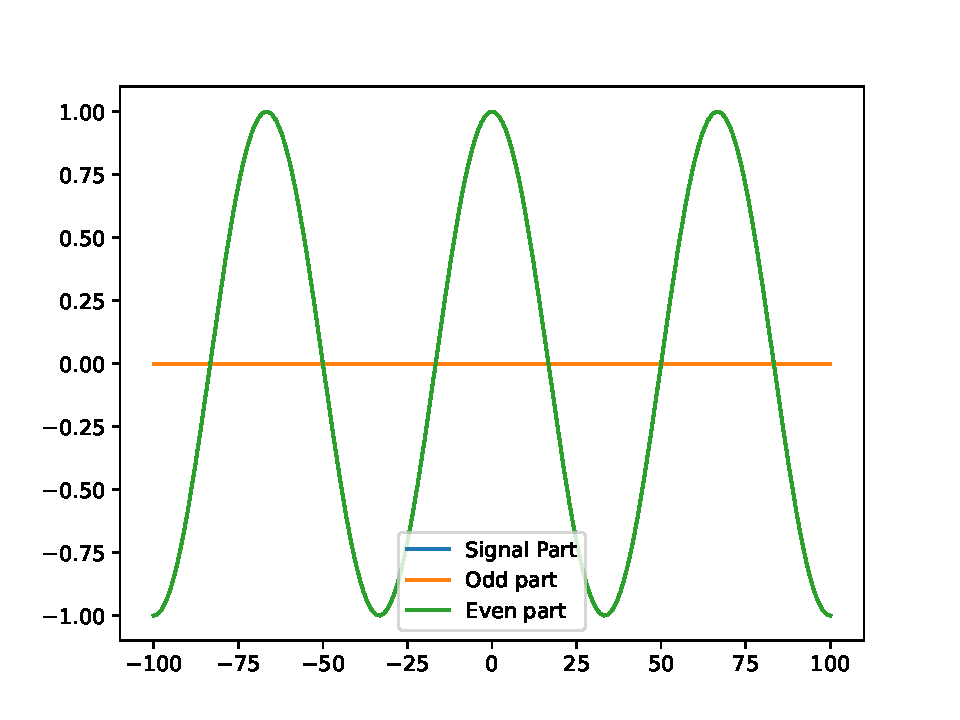
\includegraphics[scale=0.75]{a_sine.pdf}}
            \caption{sine part A}
            \end{figure}
            \begin{figure}[htp] \centering{
            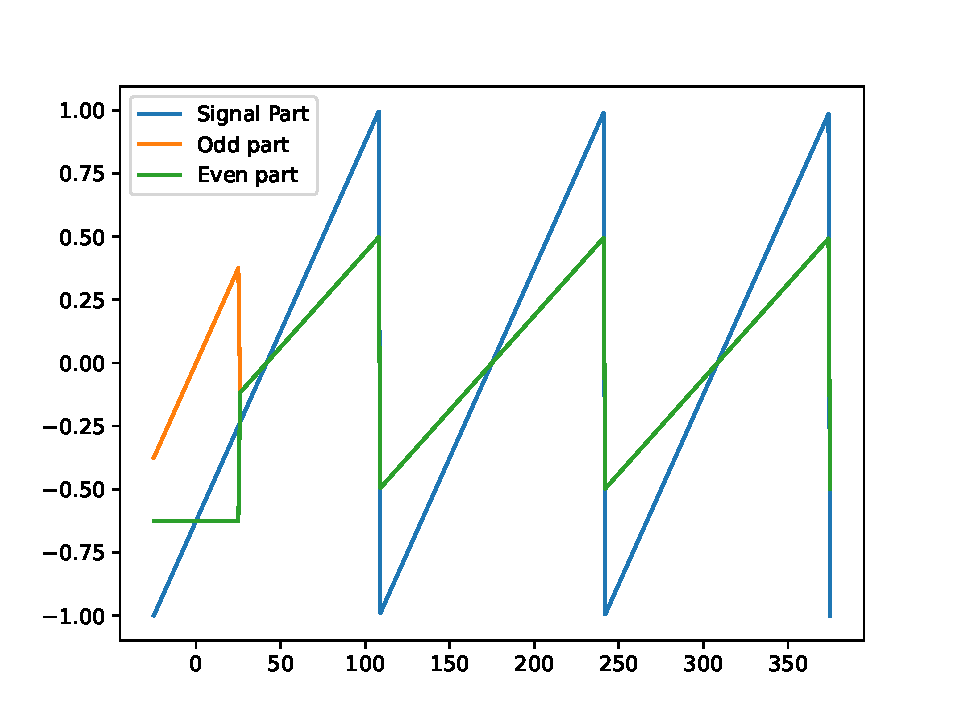
\includegraphics[scale=0.75]{a_shifted.pdf}}
            \caption{shifted sawtooth part A}
            \end{figure} 
            \begin{figure}[htp] \centering{
            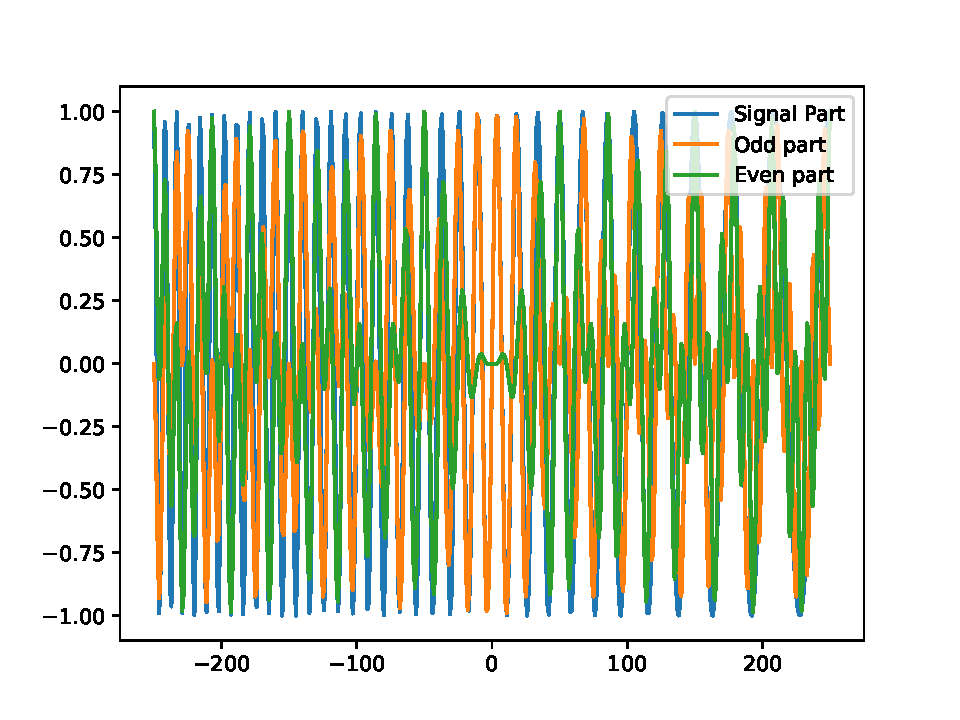
\includegraphics[scale=0.75]{a_chirp.pdf}}
            \caption{chirp part A}
        \end{figure}

\newpage
    \item %write the solution of q7b
    \begin{verbatim}
        import numpy as np
        import matplotlib.pyplot as plt
        
        # filename = "shifted_sawtooth_part_b.csv"
        filename = "sine_part_b.csv"
        # filename = "chirp_part_b.csv"
        
        data = np.loadtxt(filename, delimiter=",")
        startIndex = int(data[0])
        a = data[1]
        b = data[2]
        signalList = data[3:]
        
        n = np.arange(startIndex, startIndex+len(signalList))
        start = int(startIndex/a-b)
        end = int((startIndex+len(signalList))/a-b)
        dimension = len(signalList)/a - (end-start)
        newScale = np.arange(start-dimension, end, 1/a)
        
        plt.plot(n, signalList, label="Original signal")
        plt.plot(newScale, signalList, label="Shifted and scaled signal")
        plt.legend()
        plt.show()
    \end{verbatim}
    
    \begin{figure}[htp] \centering{
        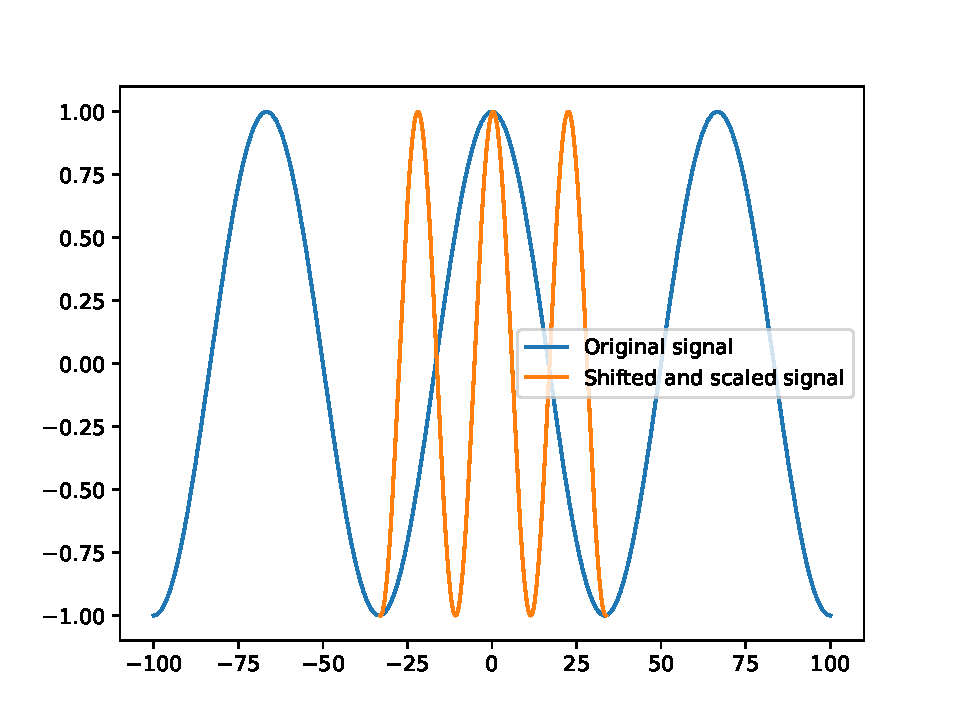
\includegraphics[scale=0.75]{b_sine.pdf}}
        \caption{sine part B}
        \end{figure}
        \begin{figure}[htp] \centering{
        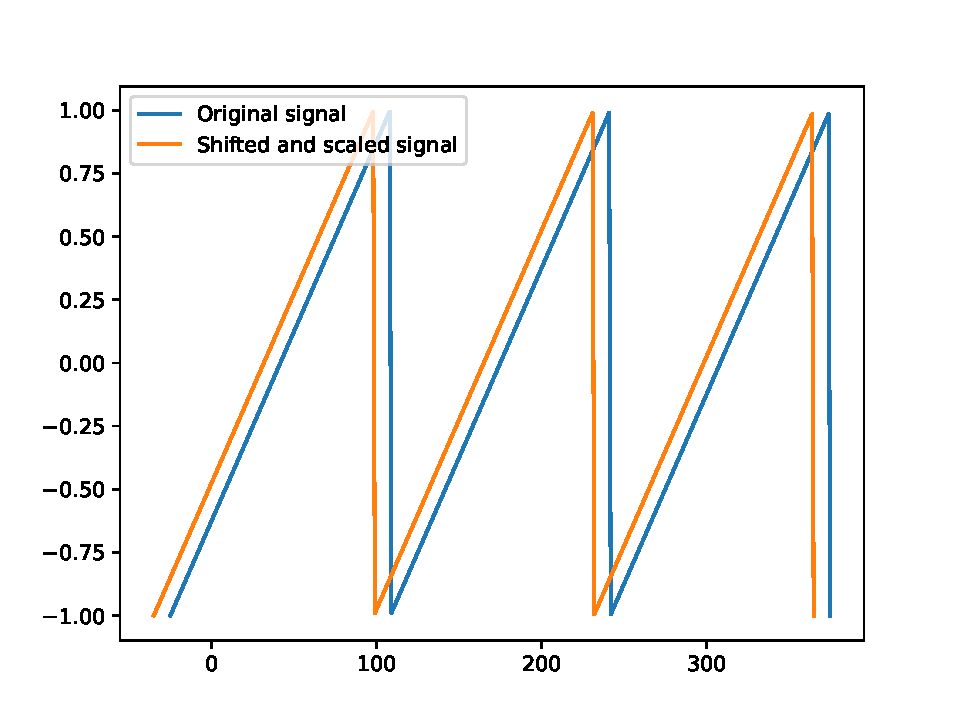
\includegraphics[scale=0.75]{b_shifted.pdf}}
        \caption{shifted sawtooth part B}
        \end{figure} 
        \begin{figure}[htp] \centering{
        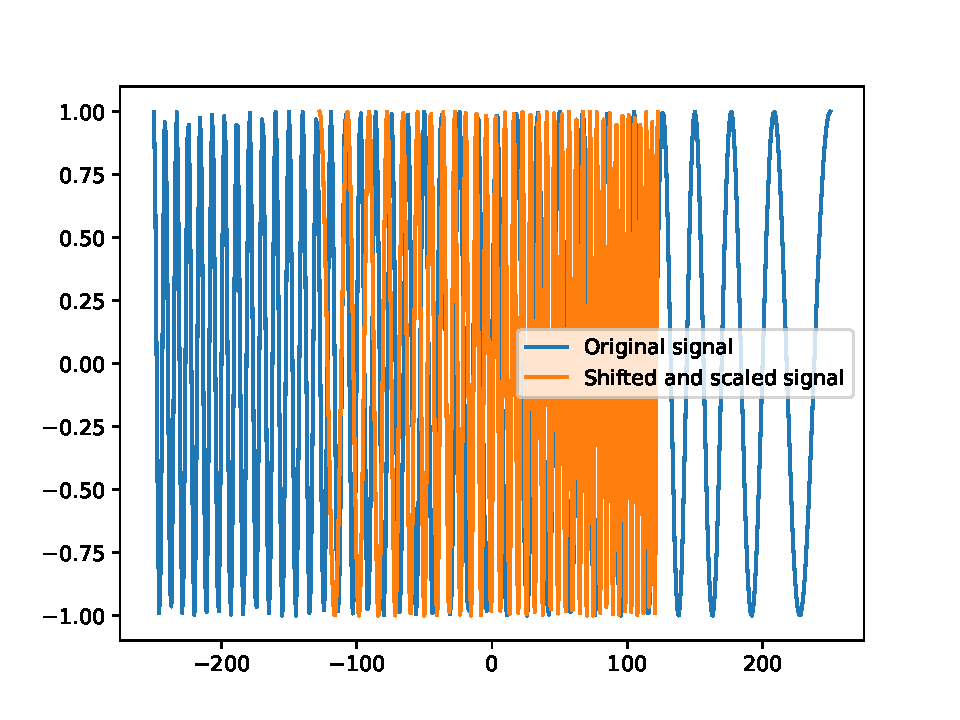
\includegraphics[scale=0.75]{b_chirp.pdf}}
        \caption{chirp part B}
    \end{figure}
    \end{enumerate}    
\end{enumerate}
\end{document}

